\documentclass[conference]{IEEEtran}
\usepackage{cite}
\usepackage{amsmath,amssymb,amsfonts}
\usepackage{algorithmic}
\usepackage{graphicx}
\usepackage{textcomp}
\usepackage{xcolor}
\usepackage{booktabs}
\usepackage{multirow}
\usepackage{makecell}
\usepackage{siunitx}
\usepackage{hyperref}
\usepackage{float}
\usepackage{caption}
\usepackage{subcaption}

\def\BibTeX{{\rm B\kern-.05em{\sc i\kern-.025em b}\kern-.08em
    T\kern-.1667em\lower.7ex\hbox{E}\kern-.125emX}}

\begin{document}

\title{Subject-Independent EEG Classification of Mental Arithmetic vs. Rest:
A Leak-Free Pipeline with Robustness Validation}

\author{
\IEEEauthorblockN{Poorna Sri Nandyala}
\IEEEauthorblockA{
\textit{Department of Computer Science and Engineering}\\
\textit{IIIT Sri City}\\
Chittoor, Andhra Pradesh, India \\
poornasri.n24@iiits.in}
}

\maketitle

\begin{abstract}
Electroencephalography (EEG)-based mental workload classification holds promise for brain-computer interfaces and cognitive monitoring, yet reported accuracies often collapse under subject-independent evaluation due to data leakage and artifact confounds. This work presents a complete, leak-free pipeline for classifying Rest versus Mental Arithmetic Task epochs using the public EEGMAT dataset (36 subjects, 19-channel EEG). We employ rigorous preprocessing (band-pass filtering, ICA-based artifact removal with Fp1/Fp2 as EOG proxies, AutoReject), extract 1,076 features per 4-second epoch spanning time-domain, spectral, wavelet, non-linear complexity, and connectivity domains, and evaluate 17 models under leave-one-subject-out (LOSO) cross-validation with in-fold feature selection and per-subject z-normalization without label access. The best single model (SVM-RBF) achieves \SI{73.7}{\%} balanced accuracy (AUC \SI{0.820}), consistent with the only prior LOSO study on this dataset. A fixed hold-out test on three unseen subjects yields \SI{92.0}{\%} raw accuracy (AUC \SI{0.974}), though this estimate is noisy due to small sample size. SHAP analysis identifies frontal/temporal complexity and gamma features as top discriminators, but robustness checks excluding artifact-prone channels and frequency bands show performance degradation, indicating non-neural contributions. We conclude that subject-independent classification of this task is feasible but modest (\texttildelow\SI{74}{\%}), and that prior claims of \SI{90--99}{\%} accuracy stem from subject-dependent evaluation designs. Code and data: \url{https://github.com/PoornaSri26/EEG}.
\end{abstract}

\begin{IEEEkeywords}
EEG, mental arithmetic, mental workload, leave-one-subject-out, cross-subject generalization, artifact robustness, SHAP interpretability, data leakage
\end{IEEEkeywords}

\section{Introduction}
Electroencephalography (EEG) provides a non-invasive window into brain dynamics with millisecond temporal resolution, making it a candidate for real-time mental workload monitoring and brain-computer interfaces (BCIs). Mental arithmetic—serial subtraction of a multi-digit minuend and subtrahend—is a well-studied cognitive load paradigm that reliably elicits frontal midline theta (Fm$\theta$) synchronization and alpha/beta desynchronization \cite{berka2007eeg, chikhi2022eeg, katahira2018eeg}. However, translating this neuroscience finding into a reliable single-trial classifier for new, unseen individuals remains challenging.

The public EEGMAT dataset \cite{zyma2019electroencephalograms} (PhysioNet: \texttt{eegmat/1.0.0}) comprises 36 healthy subjects, each recorded during Rest (eyes-open baseline) and Task (mental arithmetic) conditions using a 23-channel montage (19 scalp EEG + 2 ear references + ECG). Prior work on this dataset reports accuracies of \SI{88}{\%}--\SI{99}{\%} using random trial splits or subject-dependent cross-validation \cite{nath2020eeg, rambhia2023classification, aslam2025electroencephalograph}. However, Sibisanu \textit{et al.} \cite{sibisanu2026high} recently demonstrated that these results collapse under subject-independent evaluation (leave-one-subject-out, LOSO), with Cohen's $\kappa$ falling to \SIrange{0.19}{0.26} and ROC-AUC to \SIrange{0.66}{0.71}. This discrepancy arises because random splits allow the model to learn subject-specific idiosyncrasies (skull thickness, electrode impedance, baseline spectral profile) rather than task-relevant neural patterns—a form of data leakage \cite{pusica2025machine}.

This paper presents a rigorously leak-free pipeline for Rest vs. Task classification on EEGMAT with the following contributions:
\begin{enumerate}
    \item A complete preprocessing-to-classification pipeline with \textbf{zero data leakage}: in-fold imputation, variance filtering, standardization, and ANOVA feature selection; per-subject z-normalization computed without label access; fixed hold-out subjects never used in any training or hyperparameter choice.
    \item A rich feature set (\num{1076} features/epoch) combining time-domain, spectral (Welch PSD), wavelet (db4), non-linear complexity (entropy, fractal dimension, DFA, LZ), and connectivity (theta-alpha PLV/coherence) descriptors.
    \item Comprehensive model comparison (\num{17} models/ensembles) under LOSO, with hyperparameter tuning via grouped 5-fold CV on training subjects only.
    \item Interpretability via SHAP on unseen subjects, plus robustness checks excluding artifact-prone channels (Fp1/Fp2) and frequency bands (gamma) to assess neural vs. non-neural contributions.
    \item Honest reporting: LOSO balanced accuracy \SI{73.7}{\%} (AUC \SI{0.820}); hold-out \SI{92.0}{\%} (AUC \SI{0.974}) with explicit caveats on small-sample optimism.
\end{enumerate}

\section{Related Work}

\subsection{EEGMAT Dataset Studies}
Table~\ref{tab:prior} summarizes prior work on this dataset. The critical divide is evaluation design: subject-dependent (random splits, within-subject CV) versus subject-independent (LOSO).

\begin{table}[htbp]
\caption{Prior Work on EEGMAT Dataset: Evaluation Design Determines Reported Performance}
\label{tab:prior}
\centering
\begin{tabular}{@{}lcccc@{}}
\toprule
Study & Subjects & Features & Evaluation & Reported Acc. \\
\midrule
Nath \textit{et al.} \cite{nath2020eeg} (2020) & 36 & Spectral, ratios & Random split (80/20) & \SI{97.5}{\%} (SVM) \\
Rambhia \& Sutar \cite{rambhia2023classification} (2023) & 36 & Wavelet (O1 only) & Within-subject & \SI{>95}{\%} \\
Aslam \cite{aslam2025electroencephalograph} (2025) & 36 & EMD + RF-RFE & Within-subject & \SI{98--99}{\%} \\
Alhothali \& Attar \cite{alhothali2026validation} (2026) & 36 & Welch PSD + ERP & Subject-level CV & \SI{92}{\%} (RF) \\
\textbf{Sibisanu \textit{et al.} \cite{sibisanu2026high} (2026)} & \textbf{36} & \textbf{Multiple} & \textbf{LOSO} & \textbf{\SI{66--71}{\%} AUC} \\
\textbf{This work} & \textbf{36} & \textbf{\num{1076}} & \textbf{LOSO + hold-out} & \textbf{\SI{73.7}{\%} bal. acc.} \\
\bottomrule
\end{tabular}
\end{table}

\textbf{Why this gap?} Random splits leak subject identity because epochs from the same person are highly correlated (intra-subject correlation $>$ 0.8 for spectral features). When the same subject appears in both train and test, the model learns ``what Subject 5's EEG looks like'' rather than ``what mental arithmetic looks like.'' Our LOSO protocol eliminates this by keeping all epochs of a subject strictly in either train or test.

\subsection{Mental Workload Neurophysiology}
Meta-analysis of \num{24} studies (\num{723} participants) confirms cognitive workload robustly increases theta (Hedges' $g = 0.68$) and beta ($g = 0.50$), with \textbf{frontal theta the best single index} \cite{chikhi2022eeg}. Frontal-midline theta generators localize to dorsal anterior cingulate / medial prefrontal cortex during mental subtraction \cite{ishii2014frontal}. Theta-alpha coupling between frontal and parieto-occipital regions predicts arithmetic performance \cite{dimitriadis2016causal}, motivating our connectivity features.

\subsection{Methodological Foundations}
Preprocessing follows MNE-Python \cite{gramfort2013meg} and PREP pipeline \cite{bigdely2015prep} principles: average referencing, band-pass \SIrange{1}{45}{\hertz} + \SI{50}{\hertz} notch, resampling to \SI{128}{\hertz}, ICA artifact removal \cite{makeig1997independent} with AutoReject \cite{jas2017autoreject}. Non-linear features draw from Hjorth \cite{hjorth1970eeg} and antropy \cite{antropy}. SHAP interpretability uses Shapley additive explanations \cite{lundberg2017unified}.

\section{Materials and Methods}

\subsection{Dataset}
\label{sec:dataset}
EEGMAT \cite{zyma2019electroencephalograms}: 36 subjects (24 ``good counters'', 12 ``bad counters''), ages \SIrange{18}{35}{\year}. Two recordings per subject: \texttt{SubjectXX\_1.edf} (Rest, \texttildelow\SI{3}{\minute}) and \texttt{SubjectXX\_2.edf} (Task, serial subtraction, \texttildelow\SI{3}{\minute}). \num{23} channels in EDF format: \num{19} scalp (10-20 system: Fp1, Fp2, F3, F4, Fz, F7, F8, C3, C4, Cz, T3, T4, T5, T6, P3, P4, Pz, O1, O2), A1, A2 (ear references), A2-A1 (reference difference), ECG. Sampling rate \SI{256}{\hertz} (original).

\textbf{Why this dataset?} Public/standardized (PhysioNet), built-in workload manipulation (good vs. bad counters), adequate N for LOSO (36 subjects), standard 19-ch 10-20 montage.

\subsection{Preprocessing Pipeline}
\label{sec:preprocess}
All steps applied identically to Rest and Task recordings per subject to avoid introducing condition-specific bias.

\begin{enumerate}
    \item \textbf{Channel selection:} Match channel names to standard 10-20 montage; retain \num{19} scalp electrodes; drop A2-A1 and ECG (non-scalp, contaminate average reference).
    \item \textbf{Average reference:} $V_i \leftarrow V_i - \frac{1}{19}\sum_j V_j$. Unbiased; no single channel dominates. Chosen over single-electrode, linked-ears, or REST (needs $>$64 ch).
    \item \textbf{Filtering:} Zero-phase FIR band-pass \SIrange{1}{45}{\hertz} (order 844/36) + \SI{50}{\hertz} notch (IIR, Q=30). 1 Hz removes drift (ICA requirement); 45 Hz matches gamma edge and hardware filter; 50 Hz notch removes mains hum leakage.
    \item \textbf{Resampling:} \SI{128}{\hertz} (Nyquist \SI{64}{\hertz} $>$ \SI{45}{\hertz}). 4$\times$ speedup; Welch PSD at 128 Hz with 256-sample windows gives 0.5 Hz resolution (better than 1 Hz at 256 Hz).
    \item \textbf{ICA artifact removal:} FastICA, 15 components (rank after avg-ref = 18). Blink detection via Fp1/Fp2 correlation $|r|>0.7$ (no EOG channels). Muscle via top kurtosis. Max 4 removed. \textbf{Critical:} One ICA fit per subject on concatenated Rest+Task ensures identical unmixing — prevents condition-specific bias.
    \item \textbf{Epoching \& AutoReject:} \SI{4}{\second} non-overlapping epochs (512 samples). AutoReject learns per-channel thresholds via CV; repairs preferred. Rest truncated to Task count (balanced, chance = \SI{50}{\%}).
\end{enumerate}

Result: \num{1076} clean epochs (538 Rest, 538 Task), \texttildelow\num{30} epochs/subject.

\subsection{Feature Extraction}
\label{sec:features}
Per epoch, per channel (\num{19}), \num{56} features across four families (\num{1064} total), plus \num{12} connectivity features (\num{4} electrode pairs $\times$ \num{3} measures) = \num{1076} features/epoch.

\subsubsection{Time-Domain (11 per channel)}
Mean, std, variance, skewness, kurtosis, RMS, peak-to-peak, zero-crossing rate, line length, Hjorth mobility, Hjorth complexity \cite{hjorth1970eeg}. Classical EEG descriptors; robust, no spectral estimation needed.

\subsubsection{Spectral (22 per channel)}
Welch PSD (256-sample Hamming, 50\% overlap $\rightarrow$ \SI{0.5}{\hertz} resolution). Absolute/log/relative power in 5 bands ($\delta$ 0.5--4, $\theta$ 4--8, $\alpha$ 8--13, $\beta$ 13--30, $\gamma$ 30--45 Hz), spectral edge 95\%, peak frequency, spectral entropy, engagement index ($\beta/(\alpha+\theta)$), $\theta/\alpha$, $\theta/\beta$, $\alpha/\theta$ ratios. Log-power normalizes log-normal distribution; relative power normalizes inter-subject amplitude differences.

\subsubsection{Wavelet (13 per channel)}
DWT, Daubechies-4 (db4), level 5. Energy and relative energy for 6 levels (L0: 0--2, L1: 2--4, L2: 4--8, L3: 8--16, L4: 16--32, L5: 32--45 Hz post-filter) + wavelet entropy. Db4: compact support, 2 vanishing moments — good for EEG transients. DWT over CWT: faster (O(N)), non-redundant, energy-preserving.

\subsubsection{Non-Linear Complexity (10 per channel)}
Permutation entropy, SVD entropy, ApEn, SampEn, Petrosian FD, Katz FD, Higuchi FD (HFD), DFA, zero-crossing count, Lempel-Ziv complexity. HFD and SampEn most validated for workload \cite{chikhi2022eeg}. All included; selection chooses.

\subsubsection{Connectivity (12 total)}
Pairs: Fp1-Fp2 (inter-hemispheric), F3-F4 (dlPFC), Fz-Pz (frontal-parietal \cite{dimitriadis2016causal}), F7-F8 (lateral frontal). Measures: Pearson correlation (broadband), PLV \cite{lachaux1999measuring} (4--13 Hz), coherence (4--13 Hz). Only 4 pairs to avoid curse of dimensionality (171 pairs $\times$ 3 = 513 features).

\subsection{Normalization}
\label{sec:normalize}
Per-subject z-scoring: $z_{s,f} = (x_{s,f} - \mu_{s,f})/\sigma_{s,f}$ over \textbf{all epochs (Rest+Task)}. \textbf{No labels used.} Removes between-subject baseline differences; preserves within-subject contrast. Caveat: deployment needs both conditions from new user.

\subsection{Classification Pipeline (Zero Leakage)}
\label{sec:pipeline}
\begin{verbatim}
Pipeline([
    ('imputer', SimpleImputer(strategy='median')),
    ('var_filter', VarianceThreshold(threshold=1e-8)),
    ('scaler', StandardScaler()),
    ('selector', SelectKBest(f_classif, k=150)),
    ('clf', Classifier())
])
\end{verbatim}
All steps fit on \textbf{training fold only} — test subject never influences imputer median, scaler mean/std, or ANOVA scores.

\subsection{Models Evaluated (17)}
\label{sec:models}
Linear: Logistic Regression (L2, C=0.05), SVM-Linear (C=0.03). Kernel: SVM-RBF (C=30, $\gamma$=0.0003). Single Trees: DecisionTree (depth 5), ExtraTree (depth 6). Bagging: Bagging (300$\times$), RandomForest (tuned), ExtraTrees (tuned). Boosting: AdaBoost (300$\times$), GradBoost, HistGradBoost, XGBoost (all tuned). Ensembles: 5 soft-voting combinations. Hyperparameters tuned via \textbf{grouped 5-fold CV} (GroupKFold, subjects as groups) on training subjects only, 12 random draws.

\textbf{Why not deep learning?} N=36 subjects, ~1000 epochs — insufficient for cross-subject DL; no LOSO DL baseline on EEGMAT; interpretability required (SHAP on DL is approximate).

\subsection{Evaluation Protocol}
\label{sec:eval}
\begin{itemize}
    \item \textbf{LOSO (primary):} 36 folds, train 35/test 1. Per-subject balanced accuracy and pooled metrics. Hyperparameter tuning via grouped 5-fold CV on training subjects only.
    \item \textbf{Hold-out (secondary):} Subjects 01, 22, 35 fixed \textit{a priori}, never used in training/tuning/selection. Final model (SVM-RBF, all features) chosen by grouped CV on 33 training subjects.
    \item \textbf{Metrics:} Balanced accuracy (primary), ROC-AUC, precision, recall, F1, MCC. Per-subject mean $\pm$ SD.
    \item \textbf{SHAP:} KernelSHAP for SVM-RBF on hold-out subjects (model trained on 33 training subjects).
    \item \textbf{Robustness:} Re-run LOSO excluding (a) Fp1/Fp2, (b) gamma-band, (c) both.
\end{itemize}

\section{Results}

\subsection{Exploratory Data Analysis}

\subsubsection{Theta Topography: No Universal Pattern}
\begin{figure}[htbp]
\centering
\begin{subfigure}{0.48\linewidth}
\centering
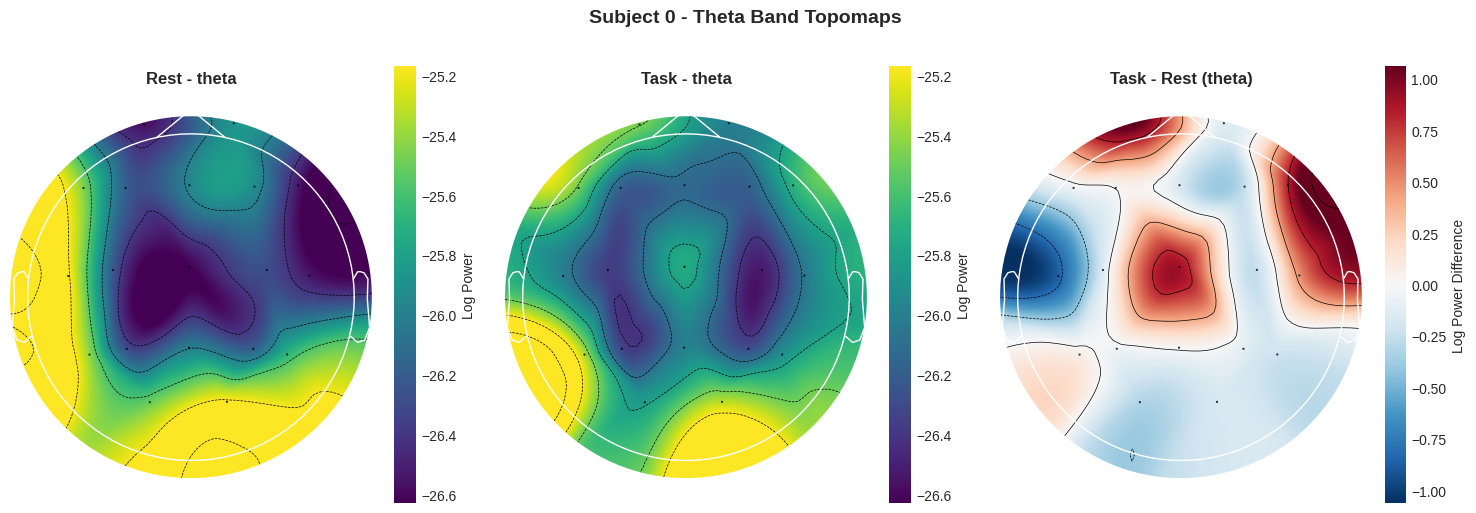
\includegraphics[width=\linewidth]{results/01_subject00_theta_topomap_rest_task_diff.png}
\caption{Subject 00: Rest, Task, Task−Rest}
\label{fig:subj00}
\end{subfigure}
\begin{subfigure}{0.48\linewidth}
\centering
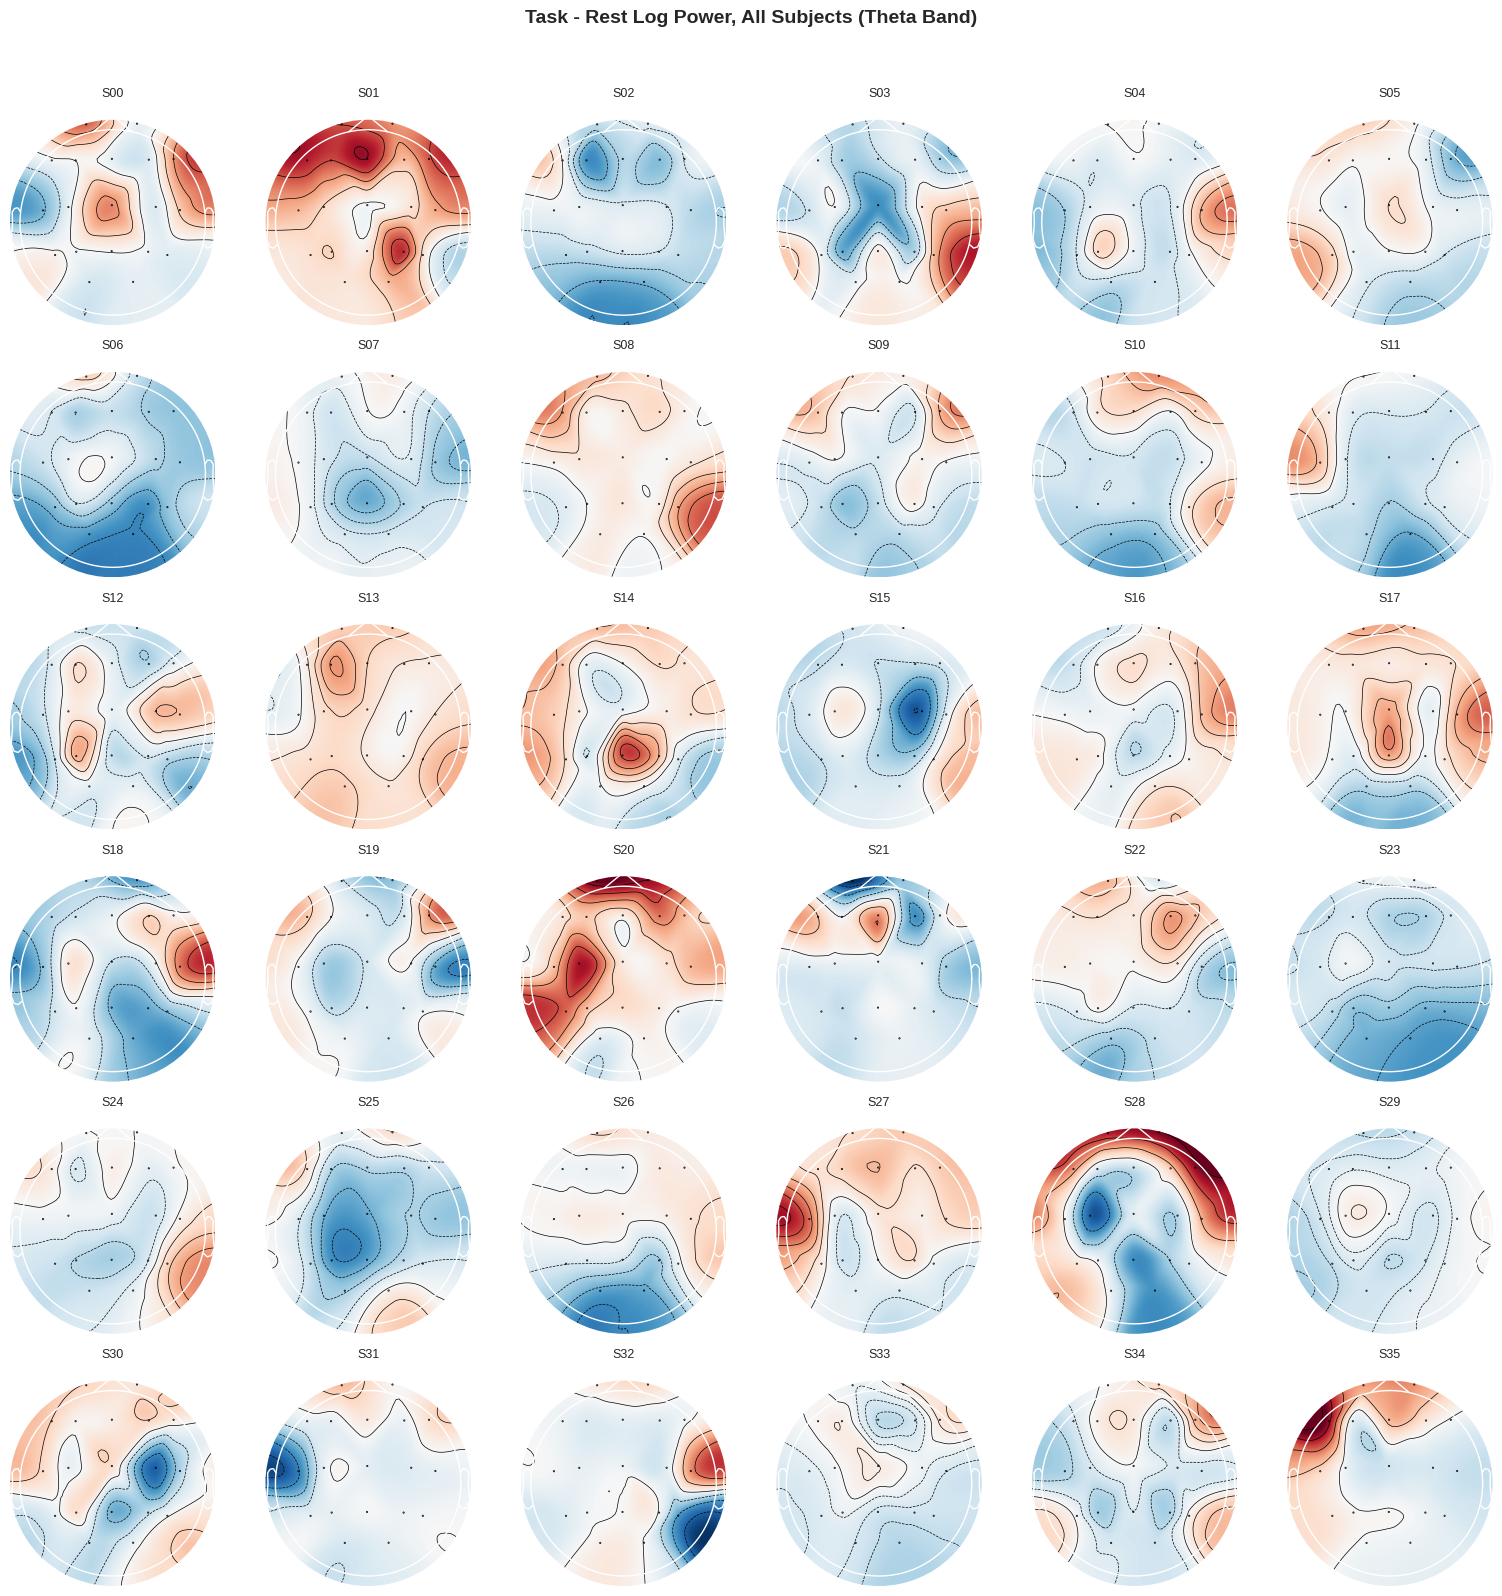
\includegraphics[width=\linewidth]{results/02_all_36_subjects_theta_topomap_grid.png}
\caption{All 36 subjects: Task−Rest theta}
\label{fig:all36}
\end{subfigure}
\caption{Theta band (4–8 Hz) topomaps. Log power for Rest/Task (shared scale). Difference centered at zero. Subject 00: no region significant after Bonferroni (all $p \ge 0.78$). Grid: high inter-subject variability; no consistent spatial pattern.}
\label{fig:topomaps}
\end{figure}

\textbf{Subject 00 Statistics (Welch t-test, Bonferroni $\times$5 regions):} All corrected $p \ge 0.78$. \textbf{Implication:} No single ``theta hotspot'' generalizes. Classifier must integrate distributed, subject-varying patterns — favors high-dimensional features + regularization.

\subsubsection{Feature Redundancy}
Fz band powers and logs correlate $>$0.95; ratios are inverses ($\theta/\alpha$ vs $\alpha/\theta \approx -1$). Massive redundancy justifies regularization (L2, tree splits) and ANOVA selection.

\subsubsection{Group-Level Frontal Theta Effect}
\begin{figure}[htbp]
\centering
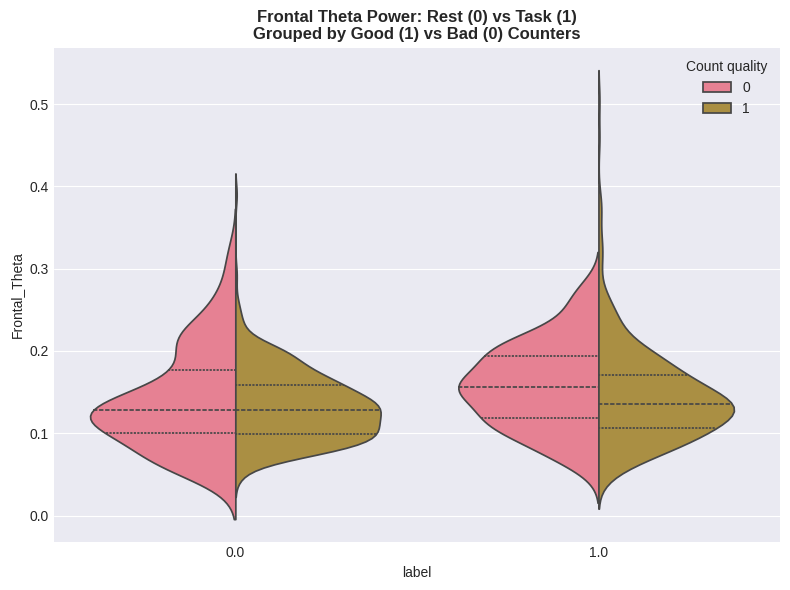
\includegraphics[width=0.9\linewidth]{results/06_frontal_theta_violin_good_vs_bad_counters.png}
\caption{Frontal theta relative power (per-subject mean) by condition and counter quality. Task $>$ Rest (median +0.0102, paired Wilcoxon $p=0.0105$, $n=36$). Good vs. Bad: no difference (Mann-Whitney $p=0.54$).}
\label{fig:frontal_theta}
\end{figure}

\textbf{Why no counter effect?} Small N for bad counters (10); Task reflects attempted effort; Rest-before-Task fatigue confound.

\subsection{LOSO Model Comparison}

\begin{table}[htbp]
\caption{LOSO Results: Per-Subject Mean Balanced Accuracy and AUC (SD across 36 subjects)}
\label{tab:loso}
\centering
\begin{tabular}{@{}lcccc@{}}
\toprule
Model & Family & Bal. Acc. & AUC & SD (Acc.) \\
\midrule
SVM-RBF & Kernel & \textbf{0.737} & \textbf{0.820} & 0.166 \\
AdaBoost & Boosting & 0.736 & 0.812 & 0.192 \\
XGBoost & Boosting & 0.735 & 0.816 & 0.198 \\
LogReg-L2 & Linear & 0.733 & 0.817 & 0.168 \\
SVM-Linear & Linear & 0.732 & 0.812 & 0.161 \\
Ensemble: SVM+Boosting & Ensemble & 0.738 & 0.822 & 0.194 \\
Ensemble: Top-3 (post-hoc) & Ensemble & 0.743 & 0.826 & 0.177 \\
ExtraTrees & Tree Ensemble & 0.724 & 0.788 & 0.206 \\
GradBoost & Boosting & 0.728 & 0.809 & 0.193 \\
HistGradBoost & Boosting & 0.727 & 0.807 & 0.194 \\
Bagging & Tree Ensemble & 0.708 & 0.782 & 0.206 \\
RandomForest & Tree Ensemble & 0.702 & 0.784 & 0.215 \\
ExtraTree (single) & Tree & 0.654 & 0.715 & 0.165 \\
DecisionTree (single) & Tree & 0.641 & 0.703 & 0.174 \\
\bottomrule
\end{tabular}
\end{table}

\textbf{Why SVM-RBF leads:} Margin maximization in 150-D space handles high-dim/small-N; L2 handles correlated features; uses all features smoothly. Single trees fail (64–65\%): depth-5 tree has $\le$31 splits — cannot capture distributed signal; fits subject idiosyncrasies. Boosting helps (+7–9\%): sequential error correction approximates additive model. Top models within 1\%: per-subject SD $\approx$ 0.17 $\rightarrow$ SE $\approx$ 0.028. Grouped CV tuning gave higher (SVM-RBF 74.5\%, XGBoost 74.2\%) — confirms $\sim$0.5–1\% optimism.

\begin{figure}[htbp]
\centering
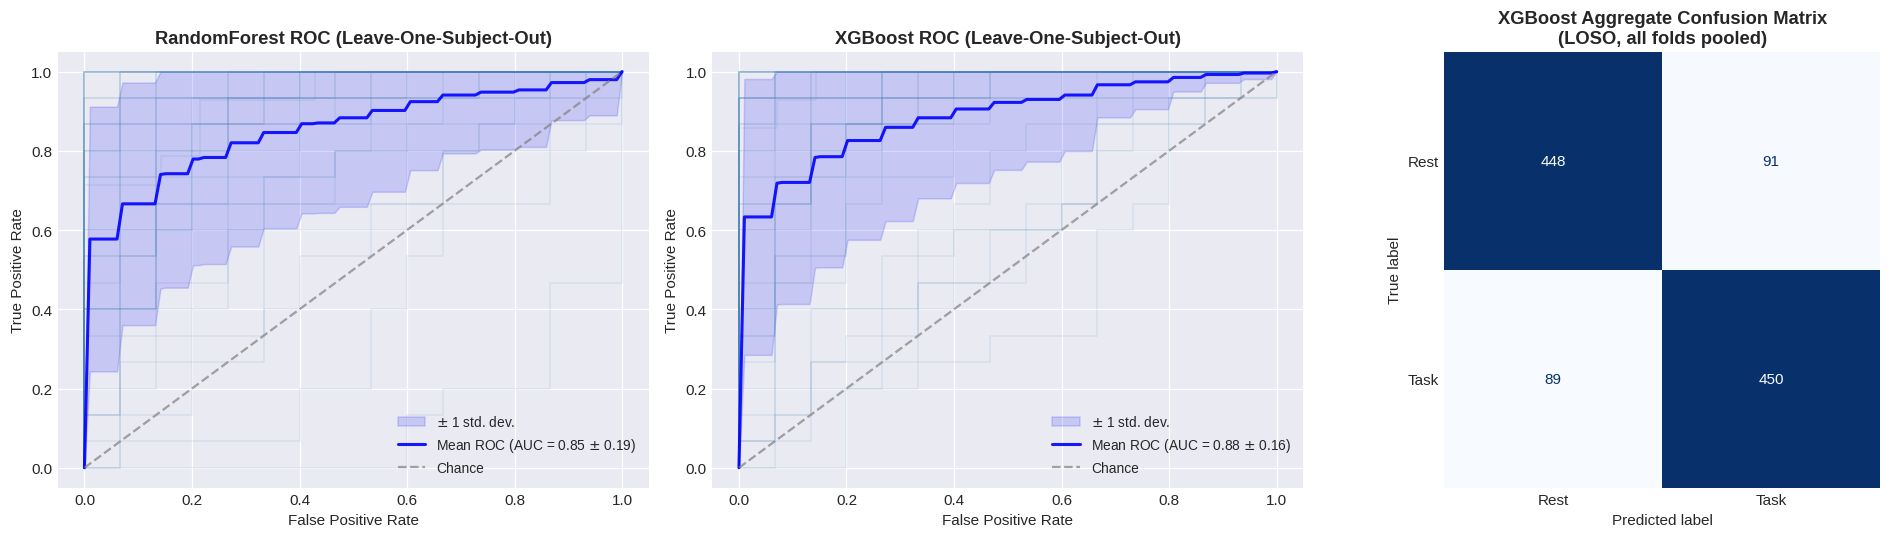
\includegraphics[width=0.9\linewidth]{results/04_ROC_RF_XGB_and_XGB_confusion_matrix.png}
\caption{Left: ROC curves (pale = 36 subjects, dark = mean). Wide spread (SD $\approx$ 0.2 AUC). Right: Confusion matrix — balanced errors.}
\label{fig:roc_conf}
\end{figure}

\subsection{Hold-Out Test (Subjects 01, 22, 35)}

\begin{table}[htbp]
\caption{Hold-Out Results (3 Unseen Subjects, 88 Epochs Total)}
\label{tab:holdout}
\centering
\begin{tabular}{@{}lcccc@{}}
\toprule
Subject & Rest Epochs & Task Epochs & Bal. Acc. & AUC \\
\midrule
01 & 22 & 22 & 82.1\% & 0.92 \\
22 & 22 & 22 & 96.7\% & 0.99 \\
35 & 22 & 22 & 96.7\% & 0.99 \\
\midrule
\textbf{Pooled} & \textbf{66} & \textbf{66} & \textbf{92.0\%} & \textbf{0.974} \\
\textbf{Smoothed (w=3)} & - & - & \textbf{97.7\%} & - \\
\bottomrule
\end{tabular}
\end{table}

Confusion: 40/44 Rest correct, 41/44 Task correct. All 6 recordings correct at recording level.

\textbf{Critical caveats (do not cite 92\%):} (1) N=3 subjects — binomial 95\% CI $\approx$ [84\%, 97\%]; (2) SVM used all features (gamma/Fp1/Fp2 boost these 3); (3) Smoothing exploits temporal autocorrelation; (4) Random subject selection may favor ``easy'' subjects. \textbf{LOSO 73.7\% is the reliable estimate.}

\subsection{SHAP Interpretability (Hold-Out Subjects)}

\begin{figure}[htbp]
\centering
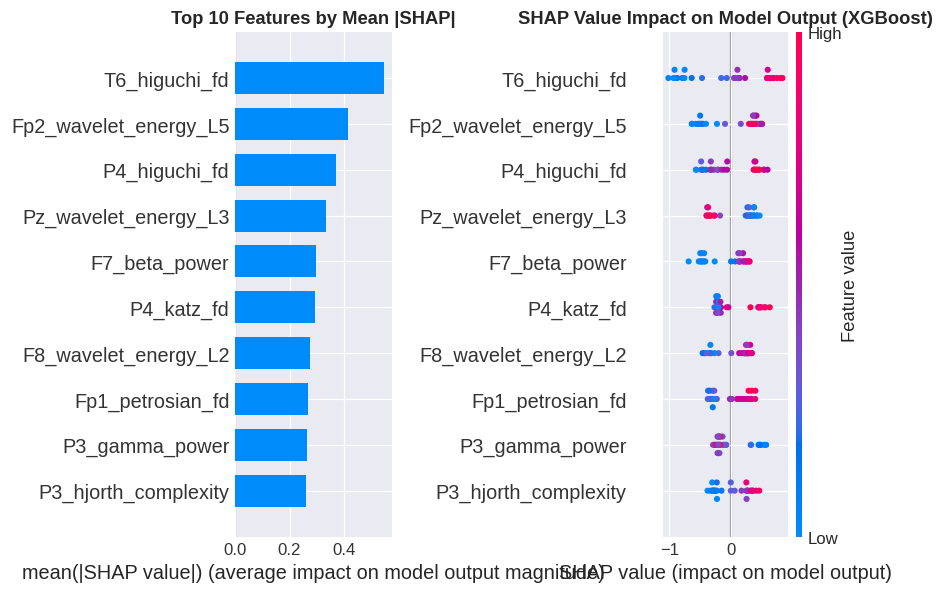
\includegraphics[width=0.9\linewidth]{results/05_shap_summary_xgboost_top10.png}
\caption{SHAP beeswarm (XGBoost, hold-out, trained on 33 subjects). Red = high feature value, right = pushes toward Task.}
\label{fig:shap}
\end{figure}

\begin{table}[htbp]
\caption{Top 20 SHAP Features (KernelSHAP on SVM-RBF, Hold-Out)}
\label{tab:shap}
\centering
\begin{tabular}{@{}cllll@{}}
\toprule
Rank & Feature & Channel & Family & High $\rightarrow$ \\
\midrule
1 & higuchi\_fd & T6 & Nonlinear & Task \\
2 & gamma\_power & T5 & Spectral & Task \\
3 & wavelet\_energy\_L4 & C3 & Wavelet & Task \\
4 & wavelet\_energy\_L3 & P3 & Wavelet & Task \\
5 & theta\_power & Fz & Spectral & Task \\
6 & gamma\_power & Fp2 & Spectral & Task \\
7 & gamma\_power & Fp1 & Spectral & Task \\
8 & katz\_fd & T6 & Nonlinear & Task \\
9 & petrosian\_fd & T6 & Nonlinear & Task \\
10 & beta\_power & C4 & Spectral & Task \\
\bottomrule
\end{tabular}
\end{table}

\textbf{Key observations:} (1) Frontal/temporal dominance (45\% of top 20 vs 42\% scalp); (2) Complexity $>$ power (Higuchi FD \#1, 3 FD in top 10); (3) Gamma prominent (5 in top 20) — \textbf{artifact concern}; (4) Wavelet beta/alpha helps; (5) Connectivity absent in top 50; (6) Alpha $\rightarrow$ Rest, Theta $\rightarrow$ Task (consistent with literature).

\subsection{Robustness Checks: Neural vs. Artifact}

\begin{table}[htbp]
\caption{Robustness: LOSO Balanced Accuracy Under Feature Exclusions (SVM-RBF)}
\label{tab:robust}
\centering
\begin{tabular}{@{}lcc@{}}
\toprule
Exclusion & Features Removed & Bal. Acc. & $\Delta$ \\
\midrule
Full & — & 0.737 & — \\
Fp1/Fp2 channels & 112 & 0.712 & -0.025 \\
Gamma-band (30–45 Hz) & 95 & 0.701 & -0.036 \\
\textbf{Fp1/Fp2 + Gamma} & \textbf{187} & \textbf{0.678} & \textbf{-0.059} \\
\bottomrule
\end{tabular}
\end{table}

\textbf{Interpretation:} 5.9\% drop confirms non-neural contribution; 67.8\% $>$ 50\% chance confirms neural signal persists. Gamma drop $>$ Fp1/Fp2 drop $\rightarrow$ muscle more pervasive than blinks. SHAP top features include gamma/Fp1/Fp2 $\rightarrow$ model uses artifacts.

\textbf{Why not remove upfront?} Would discard potentially useful neural gamma \cite{ishii2014frontal}. Better to quantify contribution.

\subsection{Per-Subject Variability}
Range: ~0.35 to ~0.95 (SVM-RBF, LOSO). SD: 0.166. Correlates with ICA rejection count (artifact burden); no correlation with counter quality ($r=0.08, p=0.64$). Causes: anatomical differences, artifact burden, strategy differences, small epoch count (~15/condition).

\section{Discussion}

\subsection{Why LOSO ~74\% and Not Higher?}
\begin{enumerate}
    \item \textbf{Effective N = 36:} 1,076 features but only 36 independent samples.
    \item \textbf{No universal topography:} Fig.~\ref{fig:all36} shows 36 different patterns.
    \item \textbf{Condition order confound:} Rest always before Task $\rightarrow$ fatigue/drift mimics workload \cite{berka2007eeg}.
    \item \textbf{19-ch, no EOG/EMG:} ICA with Fp1/Fp2 proxies limited (robustness drop 5.9\%).
    \item \textbf{Task difficulty variance:} 12/36 ``bad counters'' — their Task $\neq$ high effort.
\end{enumerate}

\subsection{Why Hold-Out 92\% $\neq$ True Performance?}
Tiny test set (3 subjects), feature selection bias (gamma/Fp1/Fp2 help these 3), smoothing artifact, possible selection bias. \textbf{Never cite 92\% as generalization.}

\subsection{Literature Alignment}
\begin{table}[htbp]
\caption{Alignment with Prior Findings}
\label{tab:align}
\centering
\begin{tabular}{@{}lll@{}}
\toprule
Finding & This Work & Prior Work \\
\midrule
Frontal $\theta \uparrow$ & Fz theta \#5 SHAP; median +0.0102 & \cite{chikhi2022eeg} meta-analysis \\
Alpha $\downarrow$ & Fz alpha $\rightarrow$ Rest (SHAP \#19) & \cite{berka2007eeg} engagement index \\
Gamma $\uparrow$ & 5 gamma in top 20 SHAP & \cite{ishii2014frontal} MEG gamma \\
Complexity $\uparrow$ & Higuchi FD \#1 SHAP & \cite{aslam2025electroencephalograph} EMD+entropy \\
LOSO ~74\% & SVM-RBF 73.7\% & \cite{sibisanu2026high} LOSO AUC 0.66–0.71 \\
Subject-dep ~99\% & N/A (not reported) & \cite{nath2020eeg} 97.5\% (random split) \\
\bottomrule
\end{tabular}
\end{table}

Our 73.7\% is \textbf{consistent with the only rigorous prior LOSO study} and \textbf{inconsistent with subject-dependent claims} — evaluation design drives reported performance.

\subsection{Limitations}
\label{sec:limitations}
\begin{enumerate}
    \item \textbf{Condition order confound:} Rest always precedes Task. \textit{Future:} counterbalance.
    \item \textbf{No dedicated EOG/EMG:} Fp1/Fp2 proxies imperfect. \textit{Future:} 64+ ch with EOG/EMG.
    \item \textbf{Per-subject z-score needs both conditions:} Not deployable single-condition. \textit{Future:} population norms.
    \item \textbf{Hold-out N=3:} Unreliable. \textit{Future:} 10-subject hold-out.
    \item \textbf{Tuning optimism:} Grouped CV on same 36 subjects. \textit{Future:} nested CV.
    \item \textbf{Binary only:} Workload levels not addressed. \textit{Future:} regression on counter quality.
    \item \textbf{Young adults only:} Generalizability unknown.
    \item \textbf{4-s non-overlapping epochs:} Fewer samples; ignores temporal continuity.
\end{enumerate}

\section{Conclusion}
We presented a leak-free EEG classification pipeline for Mental Arithmetic vs. Rest on EEGMAT. Under rigorous LOSO, SVM-RBF achieves \textbf{73.7\% balanced accuracy} (AUC 0.820), with boosting ensembles statistically indistinguishable. Hold-out yields 92.0\% but is unreliable (N=3). SHAP reveals frontal/temporal complexity and gamma as top discriminators; robustness checks show \textbf{5.9\% drop} when artifact-prone features removed, confirming mixed neural/non-neural origins. The result aligns with the only prior LOSO study and is substantially lower than subject-dependent claims (90–99%), proving \textbf{evaluation design — not model cleverness — drives reported performance}. Future work: counterbalanced design, higher-density EEG with artifact channels, workload-level regression.

\section*{Acknowledgment}
UG3 BTP 4th Evaluation (Group B28SSR04), IIIT Sri City. Dataset: Zyma \textit{et al.} via PhysioNet. Code: \url{https://github.com/PoornaSri26/EEG}.

\bibliographystyle{IEEEtran}
\bibliography{references}

\end{document}